\chapter{Příprava dat z databáze měření energetické spotřeby}

Data o měření energetické energie jsou pro pozdější analýzu nepřetržitě ukládána pomocí aplikace DEPO (kapitola \ref{aplikacedepo}) do databáze. Protože jsou data ukládána jako dlouhý řetězec znaků bez žádné pevné struktury a s proměnlivou délkou, byla pro tyto účely vybrána databáze MongoDB. 

\section{Databáze MongoDB}

MongoDB je bezplatná otevřená a platformě nezávislá databáze. Na rozdíl od většiny jiných známých typů databází pracujících s SQL příkazy, se řadí mezi takzvané NoSQL databáze. Data v databázi nejsou ukládána jako tabulky se vzájemnými relacemi, ale vkládají se jako dokumenty ve speciálním formátu podobnému formátu JSON se schématy. Díky tomu je možné do databáze vkládat data různých formátů a délek bez potřeby vytváření speciálních struktur. 

K databázi je možné přistupovat pomocí příkazů zadávaných do integrovaného terminálu, nástrojů s grafickým uživatelským rozhraním nebo použitím uživatelem vytvořených skriptů. Ke komunikaci s databází MongoDB je také možné použít sady knihoven, které jsou k dispozici pro většinu rozšířených programovacích jazyků jako jsou C, C++, Java, Python, RUBY a mnoho dalších.     

\section{Aplikace MongoDB data exporter}

Aby bylo možné dále uložená data analyzovat, například po dlouhodobém měření spotřeby, je potřeba je z této databáze získat v nějakém vhodném formátu, který je možné importovat do nástrojů jako MATLAB, Excel, OpenOffice.org Calc a podobných. Pro tyto účely byla vytvořena aplikace MongoDB data exporter. 

Aplikace MongoDB data exporter slouží jako správce databáze dlouhodobého měření energetické spotřeby robotické buňky. Kromě exportu naměřených dat ve zvoleném formátu, umožňuje vytváření záloh dat, jejich správu a čištění. 

Aplikace je napsaná v programovacím jazyce C. Pro přístup a komunikaci s databází MongoDB využívá volně dostupnou knihovnu MongoDB C Driver [\cite{}]. Protože aplikace nevyužívá žádné platformě závislé knihovny a příkazy, je možné ji zkompilovat a používat na UNIX-ových platformách i na platformě MS Windows.  

MongoDB data exporter se spouští pomocí terminálu nebo příkazového řádku. Pro jeho ovládání je použito textové uživatelské rozhraní. Během běhu programu jsou uživateli kladeny otázky, na které uživatel odpovídá ano/ne. Uživatelské rozhraní je napsáno v anglickém jazyce, pro případné rozšíření použití aplikace. Ukázka textového uživatelského rozhraní je na obrázku \ref{ukazka_run_pic}.
\\
\begin{figure}[ht]
    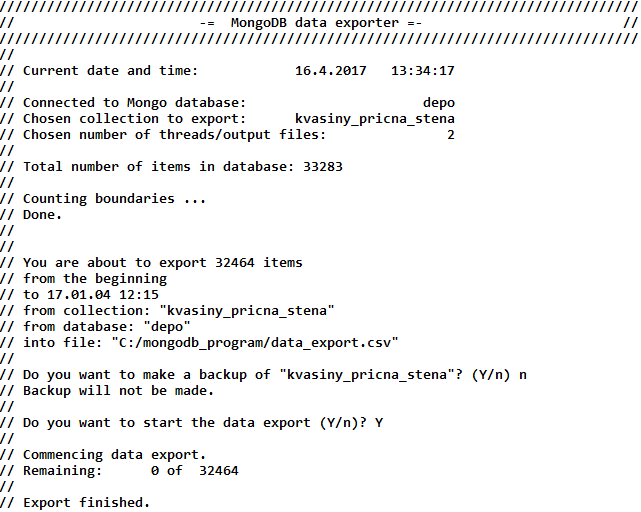
\includegraphics[width=0.9\textwidth]{ukazka_run}
    \caption{Ukázka prostředí aplikace MongoDB data exporter.}
    \label{ukazka_run_pic}
\end{figure}

Protože jsou data, pro která je aplikace určena, zpravidla získávaná dlouhodobým měřením spotřeby (v horizontu dní až měsíců), může se jejich velikost pohybovat v rámci jednotek až desítek gigabajtů. Zpracování takového množství dat může trvat dlouhou dobu. 

Pro účely urychlení a zefektivnění zpracování dat, je aplikace vytvořena jako vícevláknová. Díky tomu je možné optimalizovat využití prostředků na počítačích s vícevláknovými a vícejádrovými procesory. Každému vláknu spuštěné aplikace je přidělen svůj úsek dat, které zpracovává. Tím je docíleno paralelního zpracování několika dat současně. O přidělování prostředků a synchronizaci jednotlivých vláken se stará operační systém. Jsou použita standardní POSIXová vlákna. Počet vláken si může uživatel zvolit sám při spuštění aplikace. Aplikace podporuje až 16 vláken.       

Uživatel má dále možnosti zvolit si časový úsek, ze kterého chce data exportovat. Čas a datum od kterého a do kdy chce uživatel data exportovat se zadává s přesností na minuty. 

Data jsou standardně exportována ve formátu CSV, ale je možné použít i jiné textové formáty. Název souboru si volí uživatel. K názvu jsou dále přidané údaje o časovém úseku ze kterého jsou data exportována.

Veškerá konfigurační data jako je adresa a název databáze, použitá kolekce, počet použitých vláken, název a formát výstupního souboru pro extrakci dat a časový úsek exportovaných dat jsou čtena z textového konfiguračního souboru. Uživatel má možnost při spuštění aplikace definovat umístění a název tohoto konfiguračního souboru. 

Aby bylo možné aplikaci používat v prostředí MS Windows je nezbytné k aplikaci přiložit dynamicky linkované knihovny (DLL) potřebné pro funkci POSIXových vláken a knihoven pro práci s databází MongoDB.   

Aplikace obsahuje standardní nápovědu (help), kterou je možné spustit použitím parametru -h pri spuštění aplikace. Popis funkce a použití aplikace MongoDB data exporter je popsána v příloze \ref{}.